\section{Einleitung}
    In vielen Legierungen bildet sich zusätzlich zu der Gitterstruktur des Festkörpers eine übergeordnete
    Struktur, die sogenannte Überstruktur. Sie lässt sich in vergleichsweise makroskopischen Systemen
    über die Minimierung der Energie erreichen und ist häufig beeinflusst durch Fehlstellen und Deformationen.
    Diese Überstrukturen lassen sich beeinflussen bzw. erzeugen, sie treten nur unterhalb einer kritischen
    Temperatur auf, sodass sich durch gezieltes Erhitzen und Abkühlen eines Systems, Proben mit mehr
    oder weniger Ordnung erzeugen lassen, sodass im resultierenden Spektrum die Unterschiede zu erkennen sind.
    Im folgenden Versuch werden wir uns genau dieses Phänomen zu nutze machen, indem drei verschieden geordnete
    Proben miteinander verglichen werden. Dazu wird zunächst die röntgenographische Methode und anschließend
    das resistive Verfahren verwendet.

    \begin{figure}[H]
        \centering
        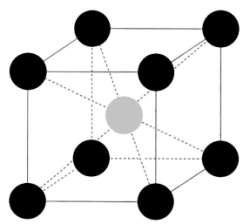
\includegraphics{images/einleitung_hurensohn.jpg}
        \label{einleitung}
        \caption{Basiszelle Cu$_3$Au [1]}
    \end{figure}